\documentclass{article}
\usepackage{amsmath}
\usepackage{amsfonts}
\usepackage{amssymb}
\usepackage{listings}
\usepackage{xcolor}
\usepackage{parskip}
\usepackage{graphicx}

\definecolor{codegreen}{rgb}{0,0.6,0}
\definecolor{codegray}{rgb}{0.5,0.5,0.5}
\definecolor{codepurple}{rgb}{0.58,0,0.82}
\definecolor{backcolour}{rgb}{0.95,0.95,0.92}

\lstdefinestyle{mystyle}{
    backgroundcolor=\color{backcolour},   
    commentstyle=\color{codegreen},
    keywordstyle=\color{magenta},
    numberstyle=\tiny\color{codegray},
    stringstyle=\color{codepurple},
    basicstyle=\ttfamily\footnotesize,
    breakatwhitespace=false,         
    breaklines=true,                 
    captionpos=b,                    
    keepspaces=true,                 
    numbers=left,                    
    numbersep=5pt,                  
    showspaces=false,                
    showstringspaces=false,
    showtabs=false,                  
    tabsize=2
}
\lstset{style=mystyle}
\usepackage[utf8]{inputenc}

\title{%
  Project 1 - Flow in a driven cavity and non conforming mesh coupling \\
  \bigskip
  \large Numerics for Fluids, Structures and Electromagnetics}

\author{Mathieu Grondin, Moritz Waldleben}
\date{January 2022}

\begin{document}

\maketitle

\section*{Introduction}
We consider the following Stokes problem on the domain $\Omega \subset
\mathbf{R}^2$ for the velocity $\mathbf{u} : \Omega \rightarrow \mathbb{R}^2$
and the pressure $p:\Omega \rightarrow \mathbb{R}$ :
\begin{align}
    \label{problem}
    -\Delta \mathbf{u} + \nabla p &= \mathbf{f}  \quad\textrm{in } \Omega\nonumber\\ 
    \textrm{div} \mathbf{u} &= 0 \quad \textrm{in } \Omega \\
    \mathbf{u} &= \mathbf{g} \quad \textrm{on } \partial \Omega  \nonumber
\end{align}
where $\mathbf{f} : \Omega \rightarrow \mathbb{R}^2$ and $\mathbf{g} :
\partial\Omega\rightarrow\mathbb{R}^2$ are two given function. In particular
assume that $\mathbf{f} \in [H^{-1}(\Omega)]^2=\mathbf{H}^{-1}(\Omega)$ and
$\mathbf{g} \in [H^{1/2}(\partial\Omega)]^2=\mathbf{H}^{1/2}(\partial\Omega)$.

This problem corresponds to solving a flow of a incompressible fluid where
viscous forces dominate inertial forces (i.e. low Reynolds number). The
equations are essentially the linearized Navier-Stokes equations neglecting
inertial terms. The dynamic viscosity is set to one in this formalation of the
problem. 

\section{Question 1}
Suppose, ab absurdo, that there exists a solution $\mathbf{u}$ to problem \ref{problem} but \\
$\int_{\partial\Omega}\mathbf{g}\cdot\mathbf{n} \neq 0$. It results that : 
\begin{align*}
    \int_{\partial\Omega}\mathbf{g}\cdot\mathbf{n} = \int_{\partial\Omega}\mathbf{u}\cdot \mathbf{n} = \int_{\Omega}\textrm{div}\mathbf{u}=\int_{\Omega}0=0 
\end{align*}
We used the fact that $\mathbf{u}$ is a solution to the equation. Furthermore
the divergence theorem was applied. This results however in a contradiction to
the assumption. Hence this proves that  $\int_{\partial\Omega}
\mathbf{g}\cdot\mathbf{n}=0$ is a necessary condition for the existence of a
solution.

From a physical point of view this correspond to the fact that there can be no
net flux outwards from the domain $\Omega$ as the flow has no source of fluid
inside the domain.

\section*{Question 2}
\subsection*{Weak formulation}
Problem \ref{problem} has to be expressed in a weak formulation. To do so we
multiply the first equation by a test function $\mathbf{v}$ and integrate over
the domain $\Omega$. Hence we get :
\begin{align*}
	& \int_{\Omega}-\Delta \mathbf{u} \,\mathbf{v}+\int_{\Omega}\nabla p \,\mathbf{v} = \int_{\Omega}\mathbf{f}\, \mathbf{v} \\
	\Leftrightarrow& \int_{\Omega} \nabla \mathbf{u} \mathbf{:} \nabla \mathbf{v}-\int_{\partial\Omega} (\nabla \mathbf{u}\cdot n)\, \mathbf{v}  -\int_{\Omega} p\, \mathrm{div}\mathbf{v}+\int_{\partial\Omega}p\,(\mathbf{v}\cdot \mathbf{n})=\int_{\Omega}\mathbf{f}\, \mathbf{v} \\
	\Leftrightarrow& \int_{\Omega} \nabla \mathbf{u} \mathbf{:} \nabla \mathbf{v}-\int_{\Omega} p\, \mathrm{div}\mathbf{v}=\int_{\Omega}\mathbf{f}\, \mathbf{v}+\int_{\partial\Omega} (\nabla \mathbf{g}\cdot \mathbf{n})\, \mathbf{v}-\int_{\partial\Omega}p\,(\mathbf{v}\cdot \mathbf{n})   
\end{align*}
In the development above we did an integration by parts and then used the fact
that $\mathbf{u}=\mathbf{g} \textrm{ on } \partial\Omega$.

Analogously we multiply the second equation by a another test function
$\mathbf(q)$ and integrate over $\Omega$ , using the same properties the
equation becomes :
\begin{equation*}
    -\int_{\Omega} q\, \mathrm{div}\mathbf{u}+\int_{\partial\Omega}q\,(\mathbf{u}\cdot \mathbf{n})=0
\end{equation*}

\subsection*{Functional spaces}
It remains the question which are the functional spaces to be imposed for the
solution of our problem. In the first equation the gradient of the
test function $\mathbf{v}$ appears. Thus we we wan't make the integral for
the test function vanish on the boundary. A natural choice is :
$[H^1_0(\Omega)]^2 = \mathbf{H}^1_0(\Omega)$
This space is formally defined by :  
\begin{align*}
	\mathbf{H}^1_0(\Omega) = \left\{\mathbf{u} \;:\; \mathbf{u} \in L^2(\Omega),
	\nabla \mathbf{u} \in L^2(\Omega), \textrm{and}
	\mathbf{u}|_{\partial\Omega}=0 \right\}
\end{align*}

Thanks to this definition on the space the two border integrals will vanish.
For the second test functions, nothing special appears, nothing more than
integral over the domain, so a natural space is $L^2(\Omega)$. 
On the other hand, for the spaces of solutions, to apply the Lax-Milgram theorem we need the
same space functions. However in this case this is not possible. First we have
a boundary condition on the border for $\mathbf{u}$. So we consider the affine
space $[H^1_g(\Omega)]^2=\mathbf{H}^1_g(\Omega)$ define as :
\begin{align*}
    \mathbf{H}^1_g(\Omega)=\left\{\mathbf{u} \;:\; u\in L^2(\Omega), \nabla \mathbf{u} \in L^2(\Omega), \textrm{ and } \mathbf{u}|_{\partial\Omega}=g \right\}
\end{align*}
For the pressure, we notice that the solution is unique up to a constant term.
To fix this we can impose that $\int_\Omega p =0$. We choose $L_0^2(\Omega)$ as
the space for pression, and we impose this space also for $q$.
\begin{align*}
    L^2_0(\Omega)=\left\{p\in L^2(\Omega)\; : \; \int_\Omega p =0\right\}
\end{align*}

The resulting problem reads :
Find $(\mathbf{u},p)\in \mathbf{H}^1_g(\Omega)\times L^2_0(\Omega)$ such that
$\forall (\mathbf{v},q)\in \mathbf{H}^1_0(\Omega)\times L^2_0(\Omega)$ the
following holds :
\begin{align}
	\label{weak_problem}
	\int_{\Omega} \nabla \mathbf{u} \mathbf{:} \nabla \mathbf{v}-\int_{\Omega} p\,
	\mathrm{div}\mathbf{v} &= \int_{\Omega}\mathbf{f}\, \mathbf{v} \\
	-\int_{\Omega} q\, \mathrm{div}\mathbf{u} &= 0 \nonumber
\end{align}

\subsection*{Mixed finite element element discrete formulation}
We will write the inifite dimensional problem in a finite dimensional
abstract form :
Find $(\mathbf{u}_h,p)\in \mathbf{V}_h(\Omega) \times Q_h(\Omega)$ such that
$\forall (\mathbf{v}_h,q)\in \mathbf{V}_{h,0}(\Omega) \times Q_{h,0}(\Omega)$ the
following holds :
\begin{align}
	\label{pert_problem}
	a(\mathbf{u}_h,\mathbf{v}_h) - b(\mathbf{v}_h,p_h) &= F(\mathbf{v}) \\
	b(\mathbf{u}_h, q_h) &= 0 \nonumber
\end{align}
The descrete case has to verify the \textbf{descrete inf-sup} condition. A
common stable choice is the mini-element which consist of an enreached
$\mathbb{P}_1$ finite element space with bubble function and
$\mathbb{P}_1$ FEM space for the pressure.

\subsection*{A priori error estimate}

\section*{Question 3}
We implemented the problem with the functional spaces given in the previous
section. The complete is shown in the annex \ref{annex}. To fix the
constant part of the pressure (we don't have any pressure boundary conditions)
we solve a slightly different problem :

Find $(\mathbf{u}^\epsilon_h,p)\in \mathbf{V}_h(\Omega) \times \mathbf{Q}_h(\Omega)$ such that
$\forall (\mathbf{v}_h,q)\in \mathbf{V}_{h,0}(\Omega) \times \tilde{Q}_h(\Omega)$ the
following holds :
\begin{align}
	\label{abstract_form_dis}
	a(\mathbf{u}^\epsilon_h,\mathbf{v}^\epsilon_h) -
	b(p^\epsilon_h,\mathbf{v}^\epsilon_h) &= F(\mathbf{v}) \\ b(p,\mathbf{v}) -
	c(p^\epsilon_h,q^\epsilon_h) &= 0 \nonumber
\end{align}

This equations are called the perturbed Stokes equations. It is simple to
verify that the zero mean pressure condition is verified. ... show that there
exists a unique solution to this problem and that the error of the perturbed
problem is not to far away from the the actual problem we wanted solve. This
strategy is called the penalty method and helps to makes the matrix formulation
of the descrete problem positive semi-definit. This property is desirable from
a computional point of view. For completness we will solve the perturbed
problem even if this is not absolutly necessary for the following questions.

In our case we know that pressures will diverge at the corners of the top
boundary when we refine the mesh. Problems thus appear mostly occur close to
the top boundary and we will define the mesh to be finer close to this
boundary. The space is divided into two rectangular regions. Specifally the
upper part will have side length of 0.1 of the total square. In each region the
mesh will have a certain number of vertices per unit length (N1 for the regions
with less interest and N2 for the other region). The ratio between N1 and N2 is
fixed to 10. The resulting mesh and solutions are depicted below:

\begin{figure}[h]
	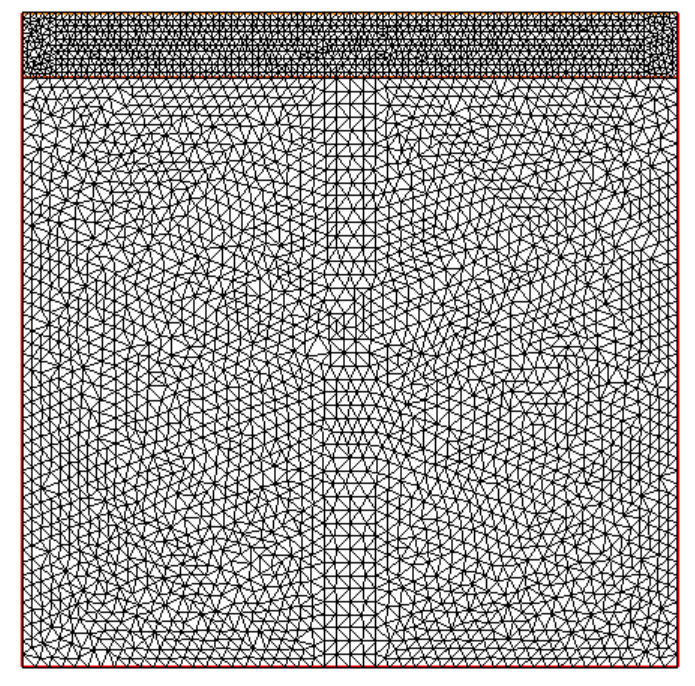
\includegraphics[width=0.5\textwidth]{imgs/Mesh_100_50.PNG}
	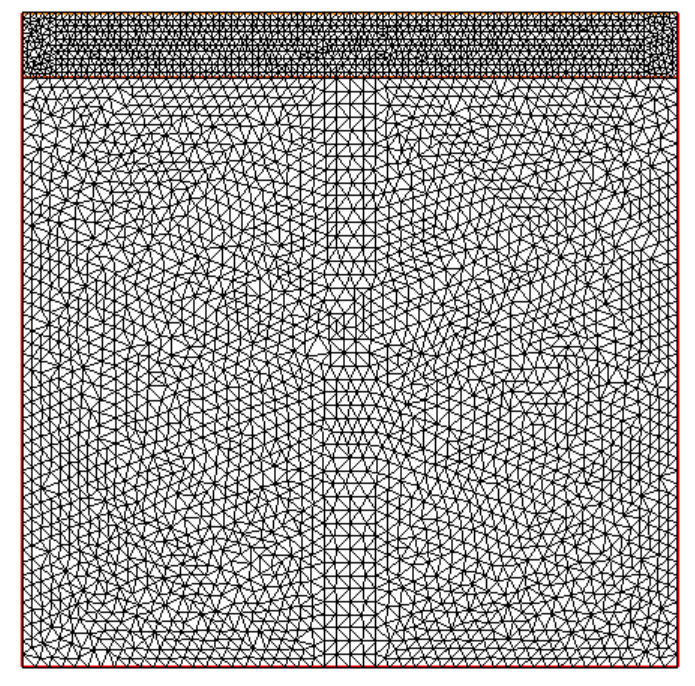
\includegraphics[width=0.5\textwidth]{imgs/Mesh_100_50.PNG}
	\caption{Conforming mesh and resulting solution using the Mini-element:
	N1=20 and N2=200}
\end{figure}

\section*{Question 4}
To reach higher accuracy, we can also use two non conforming meshes and connect
them thanks to lagrange multipliers. Due to this separation we can ask for more
precision where we need and release accuracy in the area without interest. This
is the so-called Mortar method with dual Lagrange multipliers. We implemented
this method and the code can be seen in the annex.
In contrast to the conforming problem the inerface will
contrast to the conforming case we now need two finite element spaces on two
different meshs. In addition the lagrange multipliers we needed also to define
a certain mesh and a certain finite element spaces. For the mesh it should be
the
interface between the two domains, but in FreeFEM++ this is not possible, so we
took the mesh as the border mesh of thighter mesh. For this space we used 
$\mathbf{P}_0$ for each multipliers and there is one multipliers to ensure
no discontinuities for the two axis. 

The two spaces are not defined on the same mesh. To deal with it we defined
several variationnal forms, took from those the matrix form and reconstructed
our problem as a linear system.

To see the difference between the previous method and we tested it with
different mesh sizes, the results can be seen below.

\begin{figure}[h]
	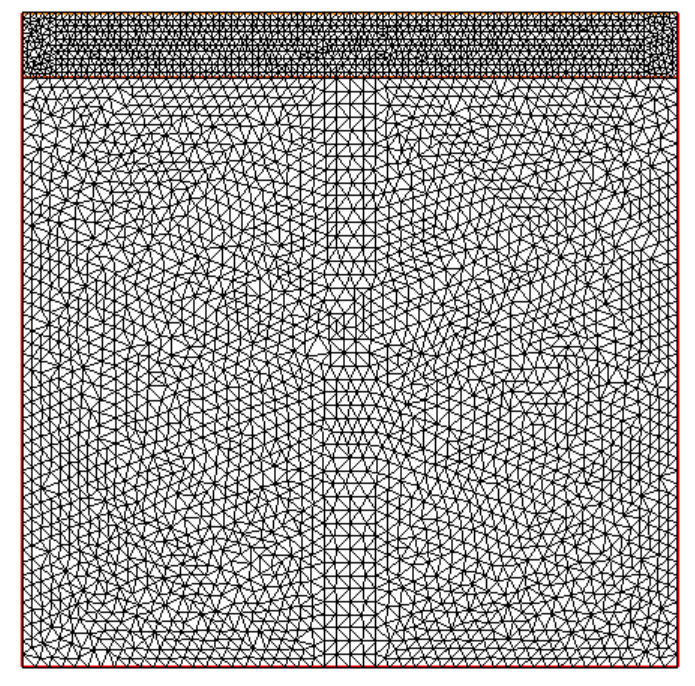
\includegraphics[width=0.5\textwidth]{imgs/Mesh_100_50.PNG}
	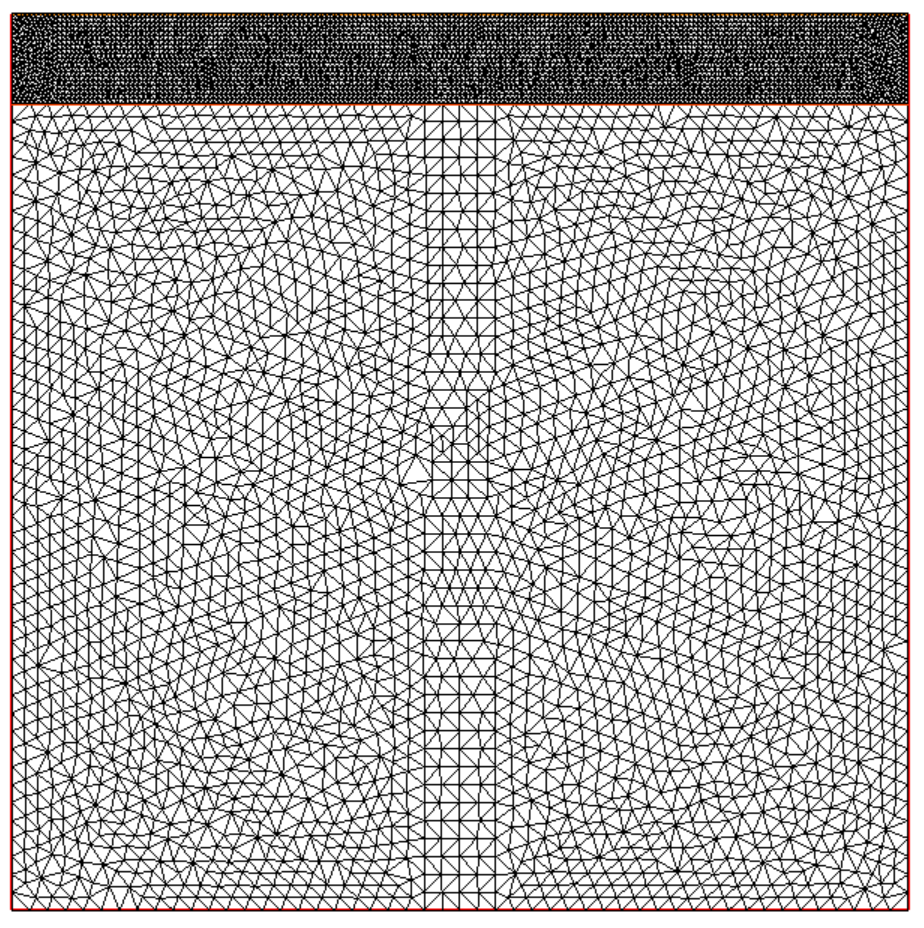
\includegraphics[width=0.5\textwidth]{imgs/Mesh_200_50.PNG}
	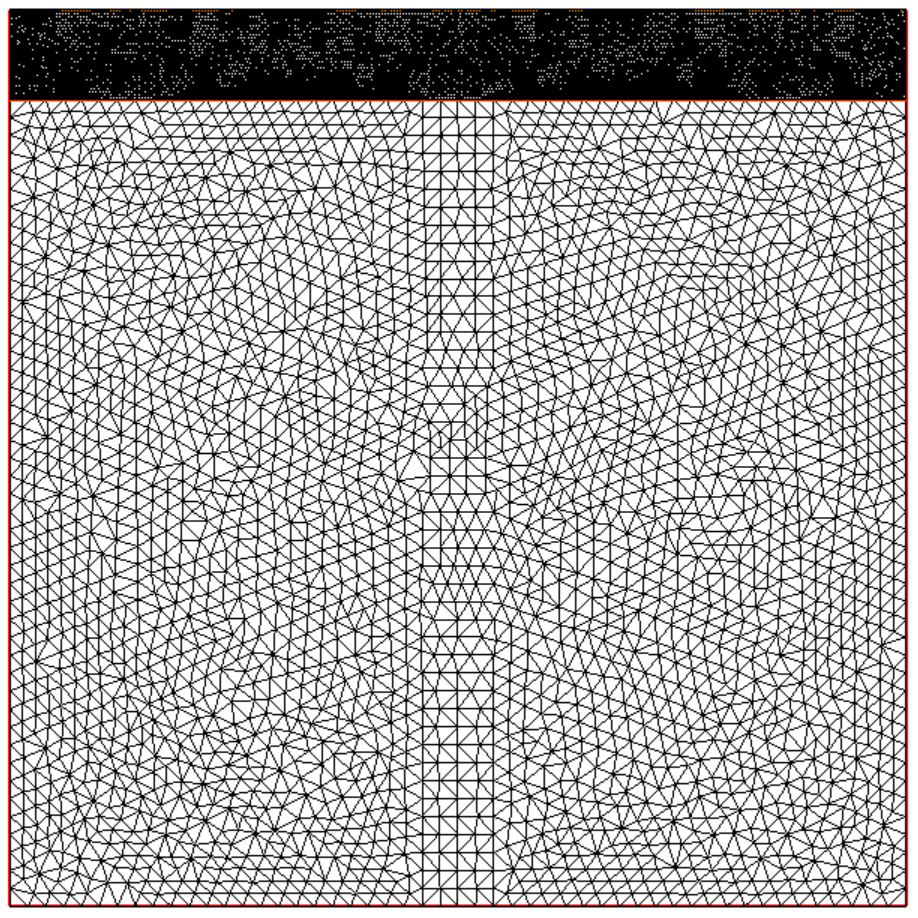
\includegraphics[width=\textwidth]{imgs/Mesh_300_50.PNG}
	\caption{Non conforming mesh with different mesh sizes: N1=50 and N2=100 (Top left), N1=50 and N2=200 (Top right) and N1=50 and N2=300 (bottom)}
    \label{fig:Meshes}
\end{figure}

After a certain coefficient, the mesh is too dense to see difference between them.

\begin{figure}[h]
	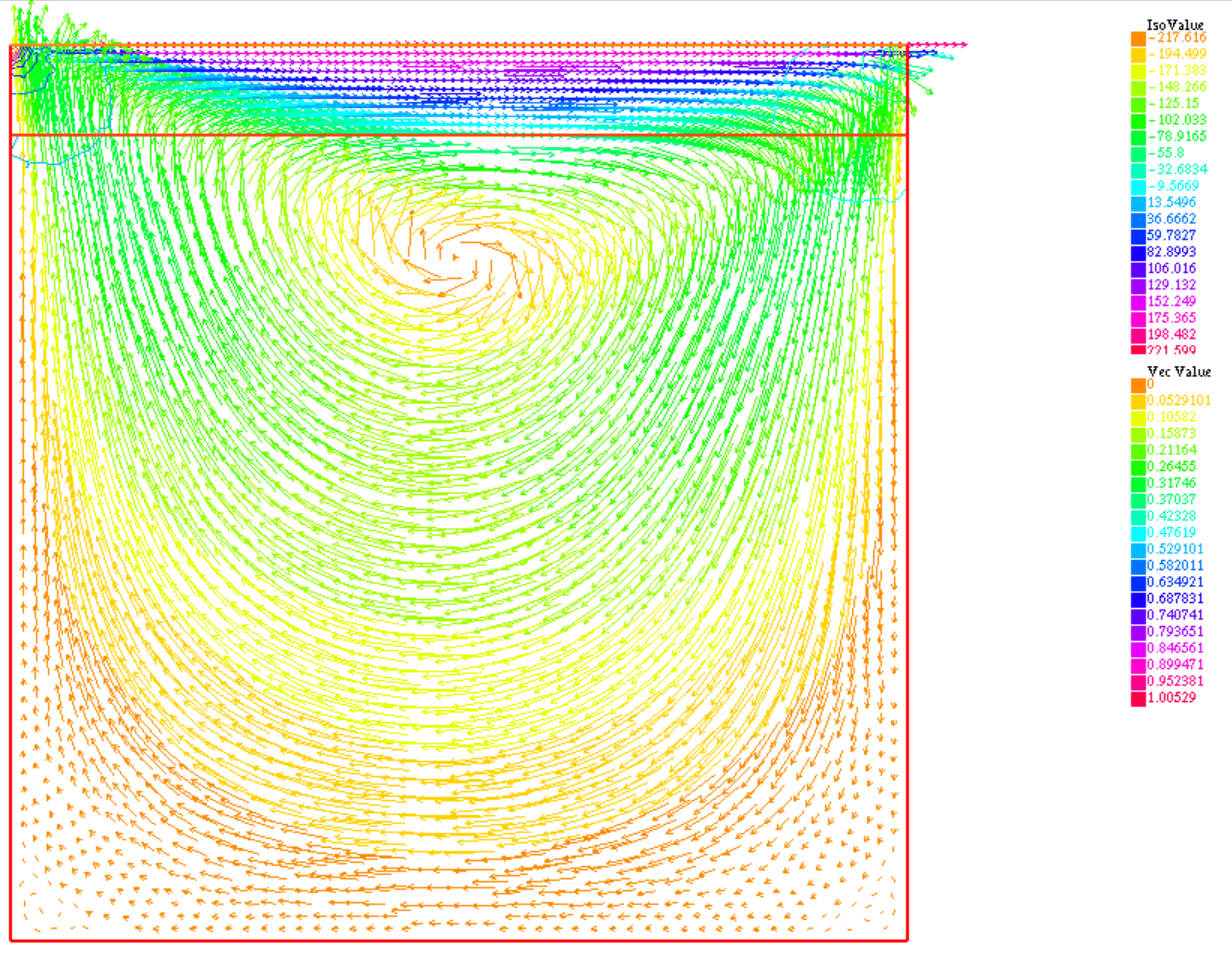
\includegraphics[width=0.5\textwidth]{imgs/solution_100_50.PNG}
	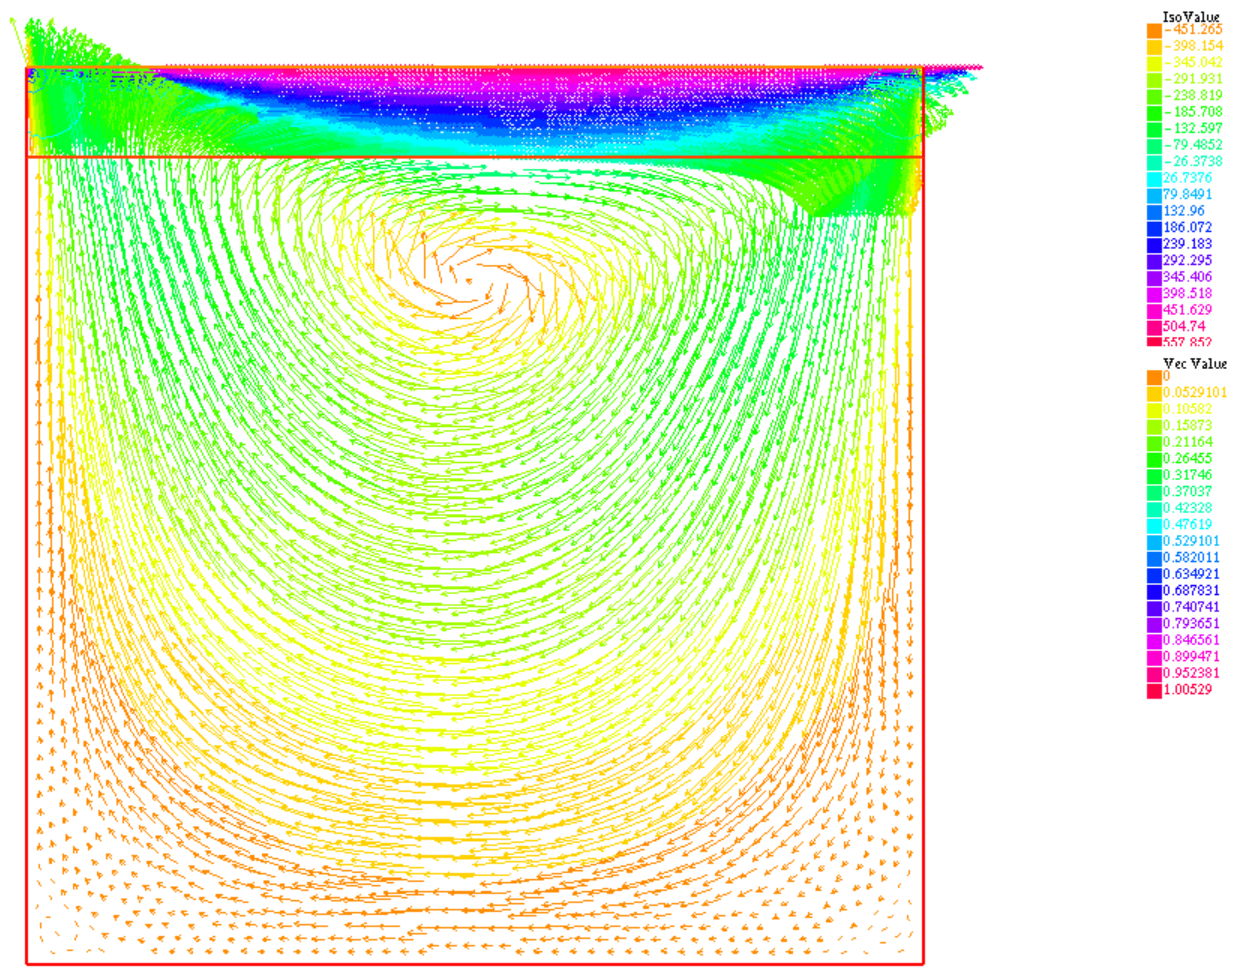
\includegraphics[width=0.5\textwidth]{imgs/solution_200_50.PNG}
	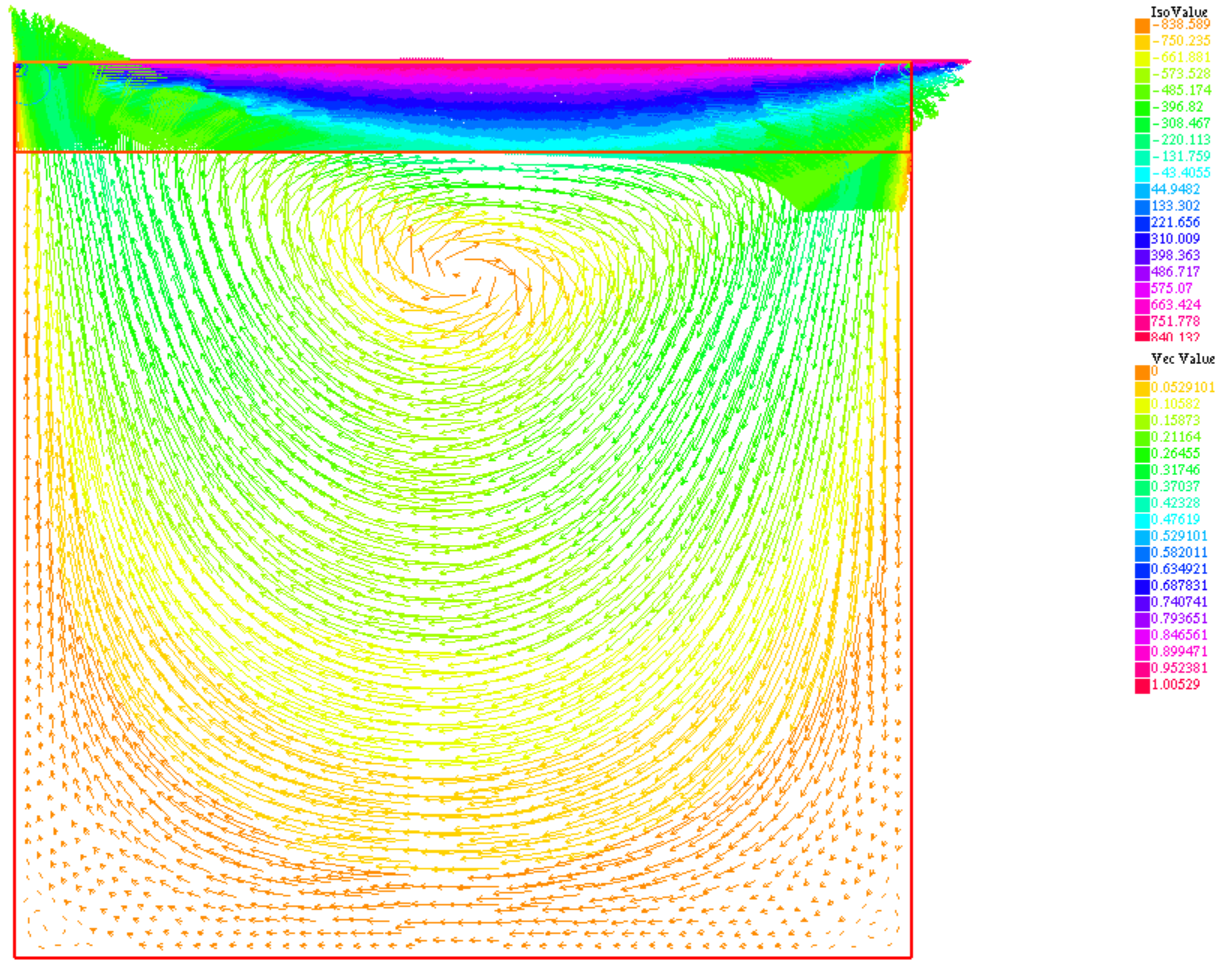
\includegraphics[width=0.5\textwidth]{imgs/solution_300_50.PNG}
	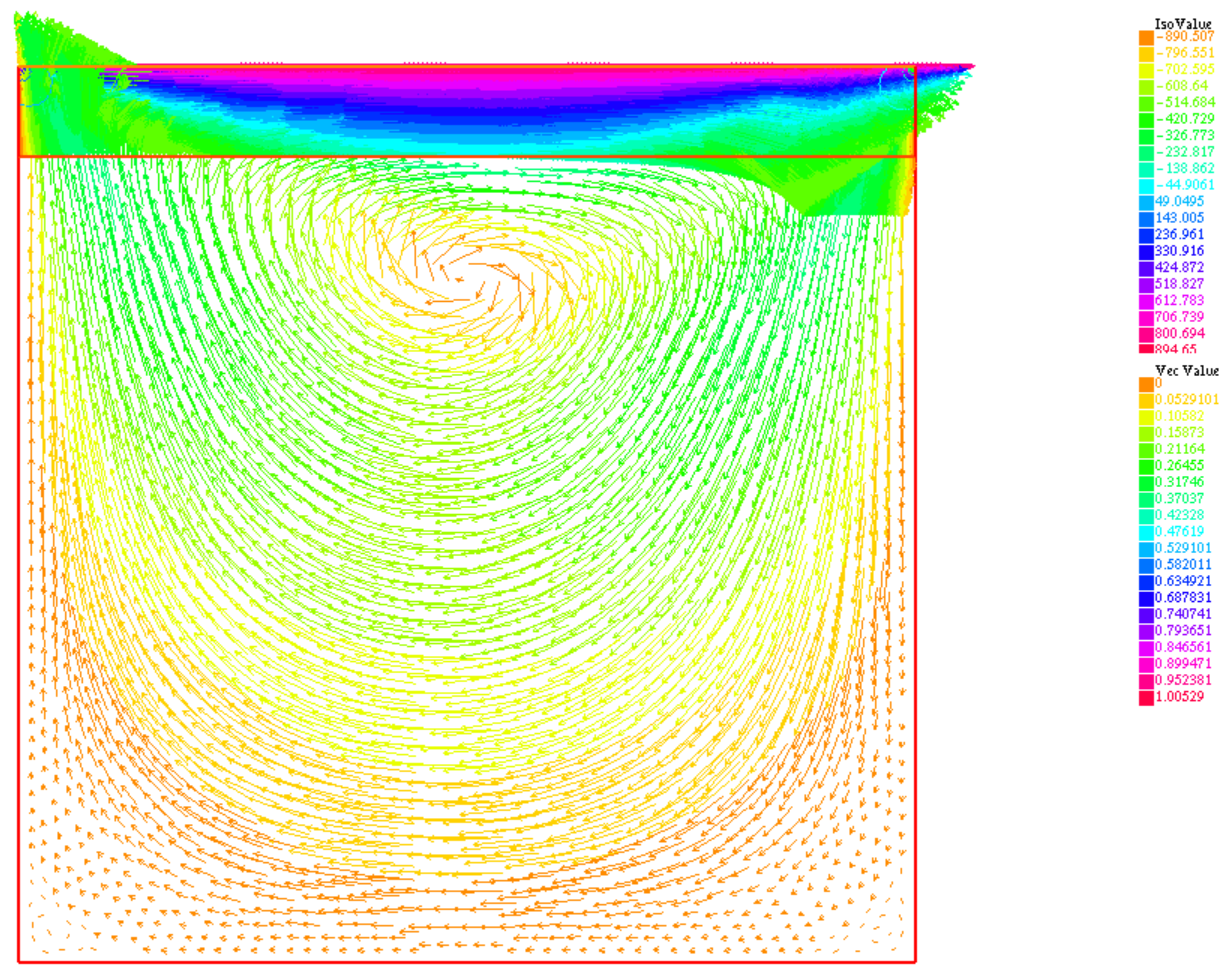
\includegraphics[width=0.5\textwidth]{imgs/solution_400_50.PNG}
	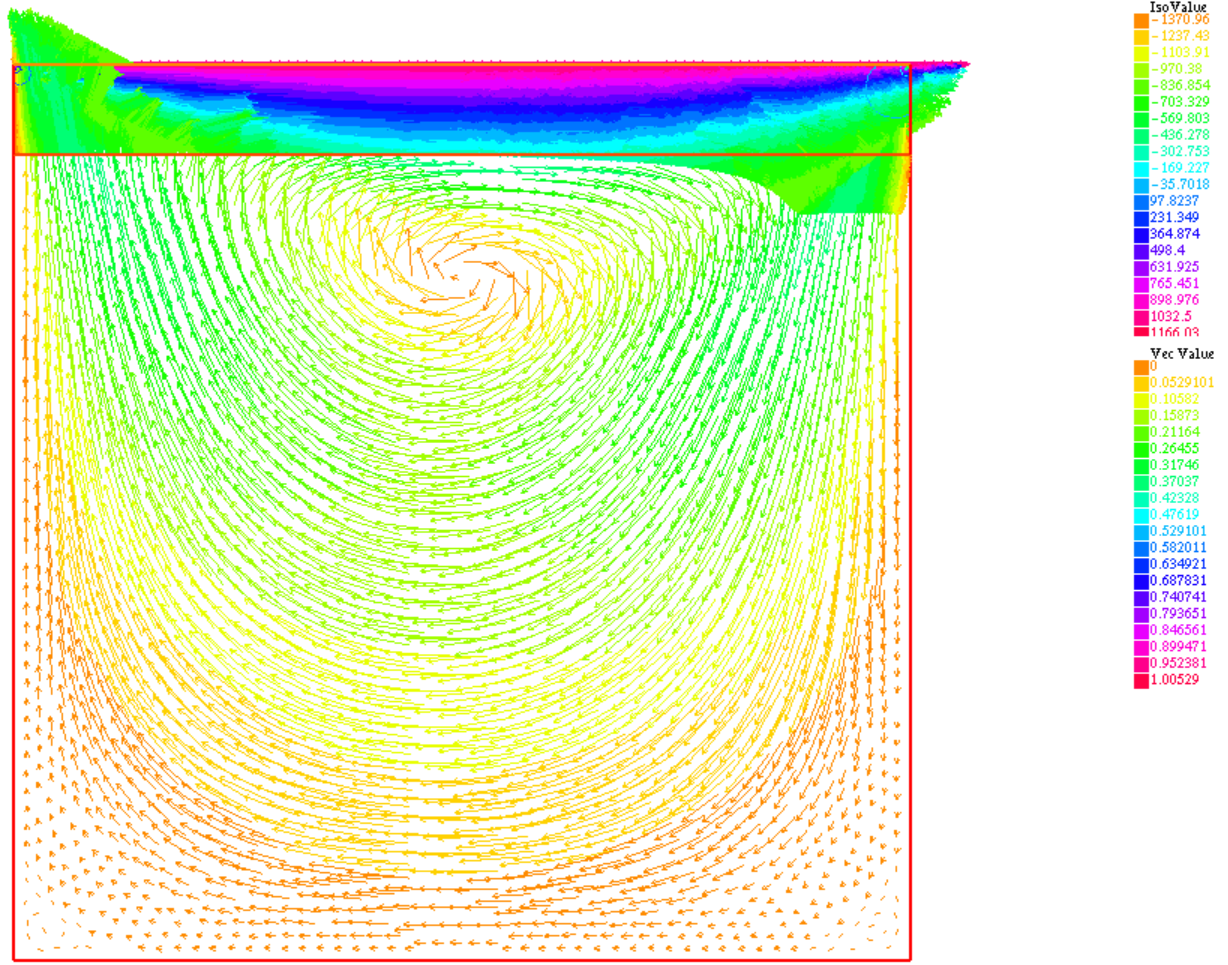
\includegraphics[width=0.5\textwidth]{imgs/solution_500_50.PNG}
	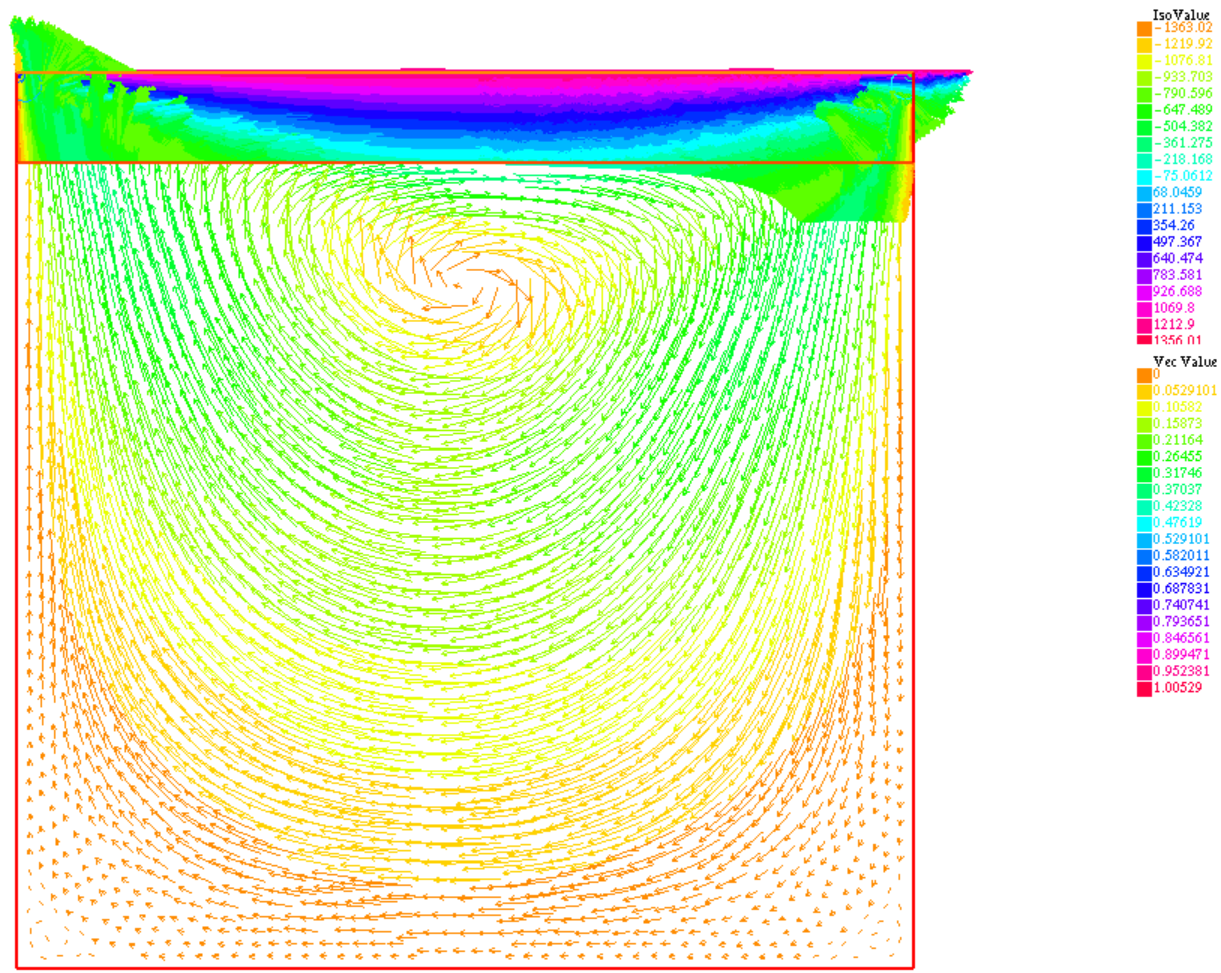
\includegraphics[width=0.5\textwidth]{imgs/solution_600_50.PNG}
	\caption{Solutions for different different mesh sizes: N1=50 and N2=100 (Top left), N1=50 and N2=200 (Top right), N1=50 and N2=300 (middle left), N1=50 and N2=400 (middle right), N1=50 and N2=500 (bottom left), N1=50 and N2=600 (bottom right)}
    \label{fig:Meshes}
\end{figure}
Comparing these results to the previous ones, we can see that the results are
similar, but we could reach higher accuracy around the interest regions. The
pressure is still diverging as expected when we refining the mesh.

\subsection*{Comparison between conforming and non-conforming meshs}
\begin{figure}
	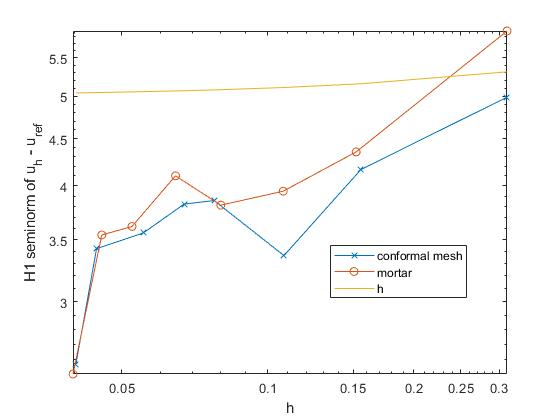
\includegraphics[width=0.5\textwidth]{imgs/errH1.jpg}
	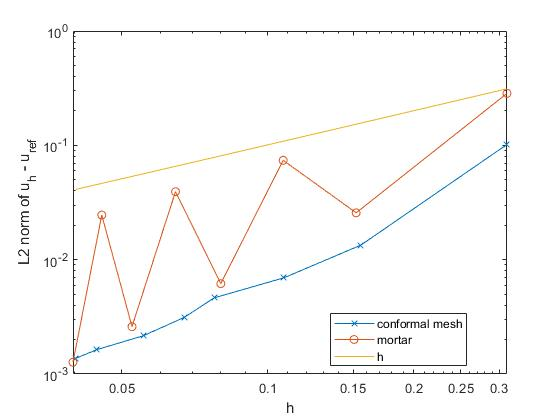
\includegraphics[width=0.5\textwidth]{imgs/errL2.jpg}
	\capture{$H^1$ seminorm and $L^2$ norm of velocity versus a reference solution, for conformal and non-conformal meshs}
\end{figure}

\section*{Question 5}

\section*{Annex} \label{annex}
Below the code for solving the stokes problem on a conforming and non conforming are shown.

\subsection*{Stokes on conforming mesh}
\begin{lstlisting} [language=C++]
	// parameters
	real eps = 1e-6; // for penalty method 

	real frac = 0.1; // fraction of side length in upper area
	int n2 = 300; // mesh size in upper area
	int n1 = n2 * frac; // mesh size in lower area

	// mesh
	border a1(t=0, 1){x=t; y=0; label=1;};
	border b1(t=0, 1-frac){x=1; y=t; label=1;};
	border c12(t=0, 1){x=1-t; y=1-frac; label=2;}; // border between areas
	border d1(t=frac, 1){x=0; y=1-t; label=1;};
	border a2(t=0, frac){x=1; y=1-frac+t; label=1;};
	border b2(t=0, 1){x=1-t; y=1; label=3;};
	border c2(t=0, frac){x=0; y=1-t; label=1;};

	mesh Th = buildmesh(a1(n1)+b1((1-frac)*n1)+c12(n1)+d1((1-frac)*n1)+a2(frac*n2)+b2(n2)+c2(frac*n2));

	plot(Th, wait=1);

	// fespaces
	fespace Xh(Th, [P1b, P1b, P1]);
	Xh [ux, uy, p], [vx, vy, q];
 	 
	// problem
	solve stokes ([ux, uy, p], [vx, vy, q])
		=   int2d(Th)(dx(ux)*dx(vx) + dy(ux)*dy(vx) + dx(uy)*dx(vy) + dy(uy)*dy(vy))
	  	  - int2d(Th)(p*(dx(vx) + dy(vy)))

      	  - int2d(Th)(q*(dx(ux) + dy(uy)))
	  	  - int2d(Th)(eps*p*q)

	  	  + on(3, ux=1, uy=0)
      	  + on(1, ux=0, uy=0);

	// plot
	plot([ux, uy], p, value=true, wait=true);
\end{lstlisting}

\subsection*{Stokes on non-conforming mesh}
\begin{lstlisting} [language=C++]
	// parameters
	real eps = 1e-6; // for penalty method 

	real frac = 0.1; // fraction of side length of upper area
	int n2 = 300; // mesh size in upper area
	int n1 = n2 * frac; // mesh size in lower area

	// lower mesh
	border a1(t=0, 1){x=t; y=0; label=1;};
	border b1(t=0, 1-frac){x=1; y=t; label=1;};
	border c1(t=0, 1){x=1-t; y=1-frac; label=2;};
	border d1(t=frac, 1){x=0; y=1-t; label=1;};

	mesh Th1 = buildmesh(a1(n1)+b1((1-frac)*n1)+c1(n1)+d1((1-frac)*n1));

	// upper mesh
	border a2(t=0, frac){x=1;y=1-frac+t; label=1;};
	border b2(t=0, 1){x=1-t; y=1; label=3;};
	border c2(t=0, frac){x=0; y=1-t; label=1;};
	border d2(t=0, 1){x=t; y=1-frac; label=2;};

	mesh Th2 = buildmesh(a2(frac*n2)+b2(n2)+c2(frac*n2)+d2(n2));

	plot(Th1, Th2, wait=1);

	// interface mesh
	mesh interface = emptymesh(Th2);

	// lower fespaces and problem
	fespace Xh1(Th1, [P1b, P1b, P1]);
	Xh1[ux1, uy1, p1];

	varf stokes1([ux, uy, p], [vx, vy, q], solver=sparsesolver)
		=   int2d(Th1)(dx(ux)*dx(vx) + dy(ux)*dy(vx) + dx(uy)*dx(vy) + dy(uy)*dy(vy))
	  	  - int2d(Th1)(p*(dx(vx) + dy(vy)))

	  	  - int2d(Th1)(q*(dx(ux) + dy(uy)))
	  	  - int2d(Th1)(eps*p*q)

	  	  + on(1, ux=0, uy=0);

	// upper fespaces and problem
	fespace Xh2(Th2, [P1b, P1b, P1]);
	Xh2[ux2, uy2, p2];

	varf stokes2([ux, uy, p], [vx, vy, q], solver=sparsesolver)
		=   int2d(Th2)(dx(ux)*dx(vx) + dy(ux)*dy(vx) + dx(uy)*dx(vy) + dy(uy)*dy(vy))
	  	  - int2d(Th2)(p*(dx(vx) + dy(vy)))

	  	  - int2d(Th2)(q*(dx(ux) + dy(uy)))
	  	  - int2d(Th2)(eps*p*q)

	  	  + on(3, ux=1, uy=0)
	  	  + on(1, ux=0, uy=0);

	// interface fespace
	fespace Ih(interface, [P0, P0]);
	Ih [lambda, mu];

	// lagrange multipliers
	varf lagrange1([lambda, mu], [ux, uy, p], solver=sparsesolver) = int1d(Th2, 2)(uy*lambda-ux*mu);
	varf lagrange2([lambda, mu], [ux, uy, p], solver=sparsesolver) = int1d(Th2, 2)(-uy*lambda+ux*mu);

	// solving
	matrix A1 = stokes1(Xh1, Xh1);
	real[int] B1 = stokes1(0, Xh1);
	matrix A2 = stokes2(Xh2, Xh2);
	real[int] B2 = stokes2(0, Xh2);

	matrix L1 = lagrange1(Ih, Xh1);
	matrix L2 = lagrange2(Ih, Xh2);
	real[int] B3(Ih.ndof); B3 = 0;

	matrix A = [[A1, 0,L1],
		    	[0, A2, L2], 
		    	[L1',L2',0]];
	set(A, solver=sparsesolver);

	real[int] B = [B1, B2, B3];
	real[int] S1(Xh1.ndof), S2(Xh2.ndof), multipliers(Ih.ndof);
	real[int] sol = A^-1 * B;
	[S1, S2, multipliers] = sol;

	p1[] = S1;
	p2[] = S2;
	lambda[] = multipliers;

	// plot
	plot([ux1, uy1], p1,[ux2, uy2], p2,value=true, wait=true);
\end{lstlisting}

\end{document}
